\documentclass[10pt,landscape]{exam}
\usepackage[phy]{template-for-exam}
\usepackage[margin=0.4in]{geometry}
\usepackage{multicol,silence,graphicx}

\WarningFilter{latex}{Label `question}
\WarningFilter{latex}{There were multiply-defined labels}
\WarningFilter{latex}{Label `part}
%%%%%%%%%%%%%%%%%%%%%%%%%%%%%%%%%%%%%

\def\todayDate{Tue, Feb 10 (Pd 1, 6) / Wed, Feb 11 (Pd 4)}

\def\content{
Write a \textbf{paragraph} explaining how the words \emph{work}, \emph{kinetic energy}, and \emph{potential energy} apply to this situation:

\vspace{1em}

\noindent
Joe is at a ski resort at the bottom of the mountain.  He rides the ski lift to the top of the mountain.  He gets off at the top, stops for a moment to admire the view, and then he skis down the mountain back to where he started.

\vspace{1em}
\noindent
  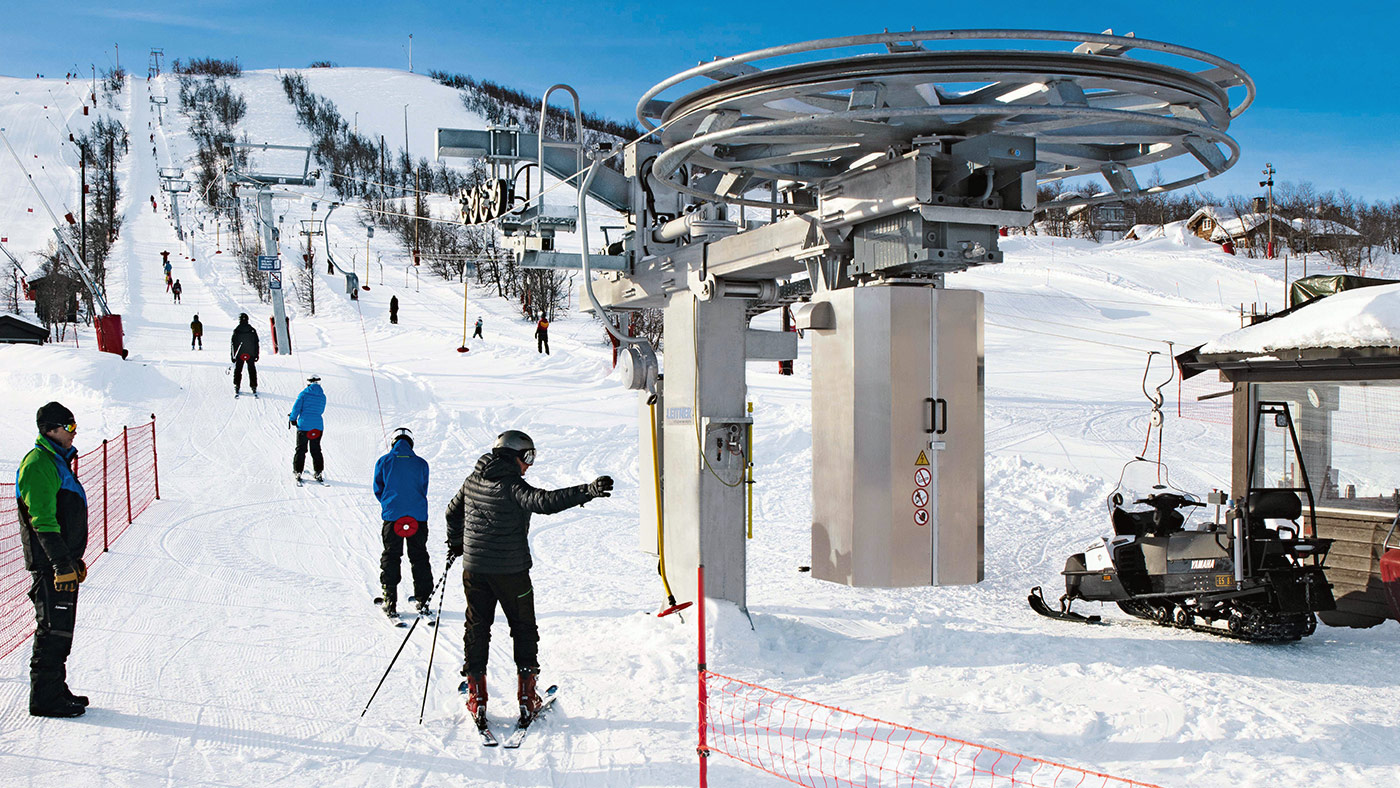
\includegraphics[width=3in]{ski.png}

}

%%%%%%%%%%%%%%%%%%%%%%%%%%%%%%%%%%%%%%

\begin{document}
\pagestyle{empty}

\setlength{\columnsep}{0.8in}
\begin{multicols*}{2}

\noindent  
Name: \hfill Period: \hspace{5em}
\vspace{0.5em}
\hrule

\section*{\todayDate}
\subsection*{Warmup}

\content

\vfill
\hrule
\vspace{0.5em}
\hfill {\sc Physics I}

\columnbreak

\noindent  
Name: \hfill Period: \hspace{5em}
\vspace{0.5em}
\hrule

\section*{\todayDate}
\subsection*{Warmup}

\content

\vfill
\hrule
\vspace{0.5em}
\hfill {\sc Physics I}

\end{multicols*}

\end{document}